\begin{flushleft}
    \section{Analysis}
        \subsection{Statement of Investigation}
            \large
            \vspace{0.2cm}
            I plan to investigate Machine Learning and Neural Networks by developing a Survival Simulation environment 
            in which a character will be controlled by a Machine Learning algorithm. \\
            \vspace{0.2cm}
            The Machine Learning Algorithm I choose to implement will most likely require lots of Complex Maths, from prior knowledge
            I know that Matrices and Calculus are heavily used within Neural Networks. Most of this Maths I will have 
            covered in my Maths and Further Maths Lessons, but some will require independant research on my Part. \\
            \vspace{0.2cm}
            The survival simulation will be procedurally generated and present multiple challenges 
            towards this character in order to provide a complex problem for it to solve. The procedural generation will
            be based upon a seed, and will generate Terrain which the character has to explore and navigate. The challenges 
            could be things like collecting items, or having to avoid/kill enemies which are actively tracking the character 
            and trying to hinder it's progress. \\
            \vspace{0.2cm}
            The key question I aim to answer with this investigation is:

            \begin{center}
                \vspace{0.3cm}
                \textbf{Can I develop a Machine Learning Algorithm to survive in a pseudorandom, open-world environment?}
                \vspace{0.3cm}
            \end{center}

            This question is rather broad and allows me to experiment with varying levels of complexity when it comes to
            the simulation. As long as I can implement a Machine Learning Algorithm which is complex enough to solve the 
            provided challenges. \\
            \vspace{0.2cm}
        \subsection{Background}
            \vspace{0.2cm}
            I am investigating Machine Learning because I've been wanting to try my hand at it for a while

            I am investigating this area of Computer Science because I've been interesting in attempting a form of
            Machine Learning for a while now but havent had a reason to dive into it. Machine Learning is an evolving
            field, with mere infinite applications such as Image Recognition, Chat Bots, Self Driving Cars, 
            etc. I feel as though my project will be sufficiently advanced enough to expand my knowledge of the subject.
            It will require lots of research, planning, and design work in order to successfully fulfil my Technical
            Solution. \\

            \vspace{0.2cm}
        \subsection{Expert}
            \vspace{0.2cm}
            For my expert I approached one of my friends, Shaun, who has prior experience with Machine Learning. He has
            created his own Hand Written Digit Recognition Network before, along with using Python Libraries such as 
            \textit{PyTorch} to train an agent to play the game \textit{Flappy Bird}, among other ML projects. He has 
            a much better understanding of Machine Learning than me currently, so hopefully he will be a good resource 
            as I develop my project. \\
            \vspace{0.2cm}
            He has agreed to answer some questions for my Interview once I have completed my Initial Investigation.
            \vspace{0.2cm}

        \subsection{First Interview}
            \large
            \vspace{0.2cm}
            As part of my Investigation I approached my friend Shaun, who has Machine Learning Experience, to give me feedback on my
            research. Along with any suggestions for my investigation. I formed a list of questions to ask him, the responses are
            paraphrased for clarity. I mainly wanted to gain an idea of what Machine Learning algorithm would suit my project the best.
            So I targetted my questions towards this.\\
            \vspace{0.2cm}
            \begin{enumerate}
                \item {\large What are your first impressions of my project?} \\
                \vspace{0.2cm}
                “Your project is definitely very complex and if finished will tick alot of the boxes needed for Full Marks. There are lots
                of layers of complexity along with room for good Object Orientated Design.”

                \vspace{0.5cm}
                \item {\large What Machine Learning Algorithms do you think would be relevant to my project?} \\
                \vspace{0.2cm}
                "Without pushing your complexity too far I think you should look into Deep Reinforcement Learning, I believe it has the
                possibility of solving your problem if not too complex. Because of that you may way want to keep your simulation as minimal
                as possible in order to give your Agent a chance. If you wanted to go further you could implement a Convolutional Neural Network, 
                but this will add to the Complexity and take more time to program."

                \vspace{0.5cm}
                \item {\large Would User Defined Parameters be helpful?} \\
                \vspace{0.2cm}
                "The ability to dynamically change the parameters through a json file or similar would be very useful. Epecially to users who
                have little to no experience with it before hand. The ability to change things like the Procedural Generation, Enemy Counts, 
                Network Structure etc would be the perfect addition to your project."

                \vspace{0.5cm}
                \item {\large What Procedural Generation method would be best for my Project?} \\
                \vspace{0.2cm}
                "I only have experience with Perlin Noise but I think that it would be a great fit for your Project. It uses simple vector Maths
                to calculate Gradient Noise, and is relatively simple to understand and Program. There are other Procedural Generation Methods
                I'm aware of like Diamond Square or Simplex Noise, but both of those are much more complicated to my understanding."

                \vspace{0.5cm}
                \item {\large How complex should I make my Simulation?} \\
                \vspace{0.2cm}
                "I would stick to a relatively simple simulation at first, and then if your agent is successful at solving it, you can add more
                to test the limits of your network after. Dynamic threats like Enemies which follow the Agent which it can attack would provide a base 
                complex problem to start off with. Other problems could be collecting items or a simple Food Collection system with a Hunger Meter."

                \vspace{0.5cm}
                \item {\large How should I determine if my project is successful?} \\
                \vspace{0.2cm}
                "You could log a graph of Loss compared to Time, and in theory if your agent is learning it will successfully reduce the average Loss 
                the more training it receives. You could use this graphed data as supporting evidence in your Evaluation."

                \vspace{0.5cm}
                \item {\large What should I focus my Initial Research on?} \\
                \vspace{0.2cm}
                "It would be benefical to you to research the Maths behind Neural Networks, specifically for Forward Propagation
                and Back Propagation. The Maths behind it can get very complicated, along with being very hard to debug if a small error is made.
                They both heavily rely on Matrix Operations, so if you're not familiar with those you should get up to speed."

                \vspace{0.5cm}
            \end{enumerate}
            
        \subsection{Initial Research}
                \subsubsection{Existing Investigations} 
                    \paragraph{Crafter} \mbox{} \\
                        \vspace{0.2cm}
                            In my research on the Internet I discovered a project called $Crafter$. \\

                            \vspace{0.2cm}
                            \centerline{\textit{https://github.com/danijar/crafter}}
                            \vspace{0.2cm}

                            Crafter is described to be \textit{"Benchmarking the Spectrum of Agent Capabilities"}, and is utlised
                            in conjunction with Machine Learning Algoriths such as $DreamerV2$, $PPO$ and $Rainbow$. Crafter poses significant
                            challenge towards its Player, requiring high levels of generalisation, long-term reasoning, and complex 
                            problem solving. If the machine Learning algorithm in question fails to achieve one of these aspects it will 
                            struggle to full "Solve" the simulation. \\

                            \vspace{0.2cm}

                            High levels of generalisation are required when training a Machine Learning algorithm, if this is not achieved then
                            your network will only lend itself to a single Dataset/Problem. An example of this would be training a network used
                            to recognise hand written digits on only one way of writing 4's, if presented with an input for a different type of 
                            4 it may not recognise it and identify it incorrectly. \\
                            
                            \vspace{0.2cm}

                            Long-Term reasoning is a complex problem to solve in the context of Machine Learning, current Machine Learning models
                            struggle to deal with this problem. This is dealt with by using algorithms built to mimic "memory". A common 
                            implementation of this is Experience Replay which stores states in a queue, and relearns from it after every N ammount
                            of steps. \\

                            \vspace{0.2cm}

                            A complex reward and action system may take time for an algorithm to learn but it certainly is possible with current
                            Machine Learning Models. Crafter utilises a complex action system with a flow chart determining which Action can be taken
                            given the current state of the simulation. Below is shown the Complex Flow Chart of Actions: \\

                            \vspace{0.2cm}
                            \begin{center}
                                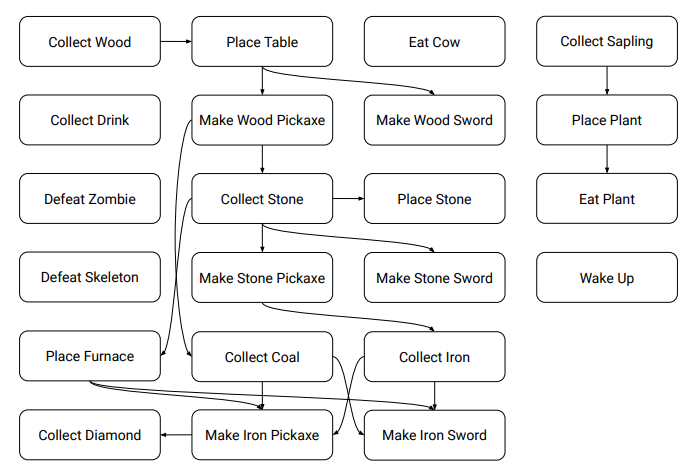
\includegraphics[width=12cm]{Images/InitialResearch/CrafterComplexActionSystem.PNG} \\
                                Complex action system as shown in the Paper "Benchmarking the Spectrum of Agent Capabilities" \\
                            \end{center}
                            \vspace{0.2cm}

                            Crafter manages to achieve quite high success rates with various Algorithms, but they still fail to overcome, or even match
                            human standards. This is likely due to the complexity of the problem, and in theory will be solvable within the near future
                            as Machine Learning advances over the next few years. This is why I plan to create a simpler simulation which the Agent will
                            be more likely to be able to solve. Below is shown the Success Rate Data for both Algorithms and Human Experts. \\

                            \vspace{0.4cm}
                            \begin{figure}
                                \centering
                                \subfloat[\centering Success Rate of Algorithms]{{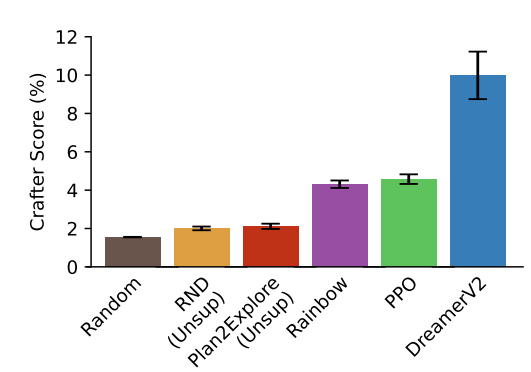
\includegraphics[width=7cm]{Images/InitialResearch/CrafterMLTrainingData.PNG}}}
                                \qquad
                                \subfloat[\centering Comparison Against Human Data]{{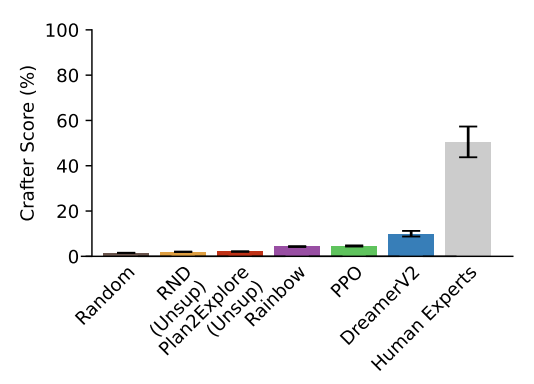
\includegraphics[width=7cm]{Images/InitialResearch/CrafterMLTrainingData+Human.PNG}}}
                            \end{figure}
                            \vspace{0.2cm}

                            While I would love to create a simulation similar to crafter, it is very complex and would take a long time to develop. Yet
                            would not net many marks in the process. Overall I feel like Crafter is a good example that my project is possible, but will
                            require a complex Machine Learning Model in order to achieve reliable results from my Investigation.

                        \vspace{1cm}
                    \paragraph{Minecraft} \mbox{} \\
                        \vspace{0.2cm}
                        Minecraft is a \textit{very} popular Game. It's a sandbox game, meaning that the player can do almost anything they want.
                        The game is formed from blocks which can be broken or placed, along with a plethera of items, enemies, passive animals
                        and more. It has infinite terrain generation, and explicity uses Perlin Noise, and is generated from a seed. The seed determines
                        all the terrain generation, loot tables, random structures, caves, etc. \\
                        
                        \vspace{0.2cm}

                        First it starts off on a very broad level, painting a basic topographical map of the world. It uses Perlin Noise to sample
                        a height value for each chunk, where chunks are 16x16 areas of blocks. Then within these chunks the game uses the Diamond Square
                        algorithm to interpolate between it and the chunks around it, creating blocks where the terrain should be. This produces an 
                        entirely deterministic results based upon the seed.\\

                        \vspace{0.2cm}

                        Secondly, the Caves are generated using Perlin Worms, which travel in deterministic directions based on their starting position.
                        These worms dig through the terrain carving out caves which can then be traversed by the player. Within these Caves spawn water
                        sources, pools of lava, useful ores. All of these are deterministically generated by the original seed. \\ 

                        \vspace{0.2cm}
                        \begin{center}
                        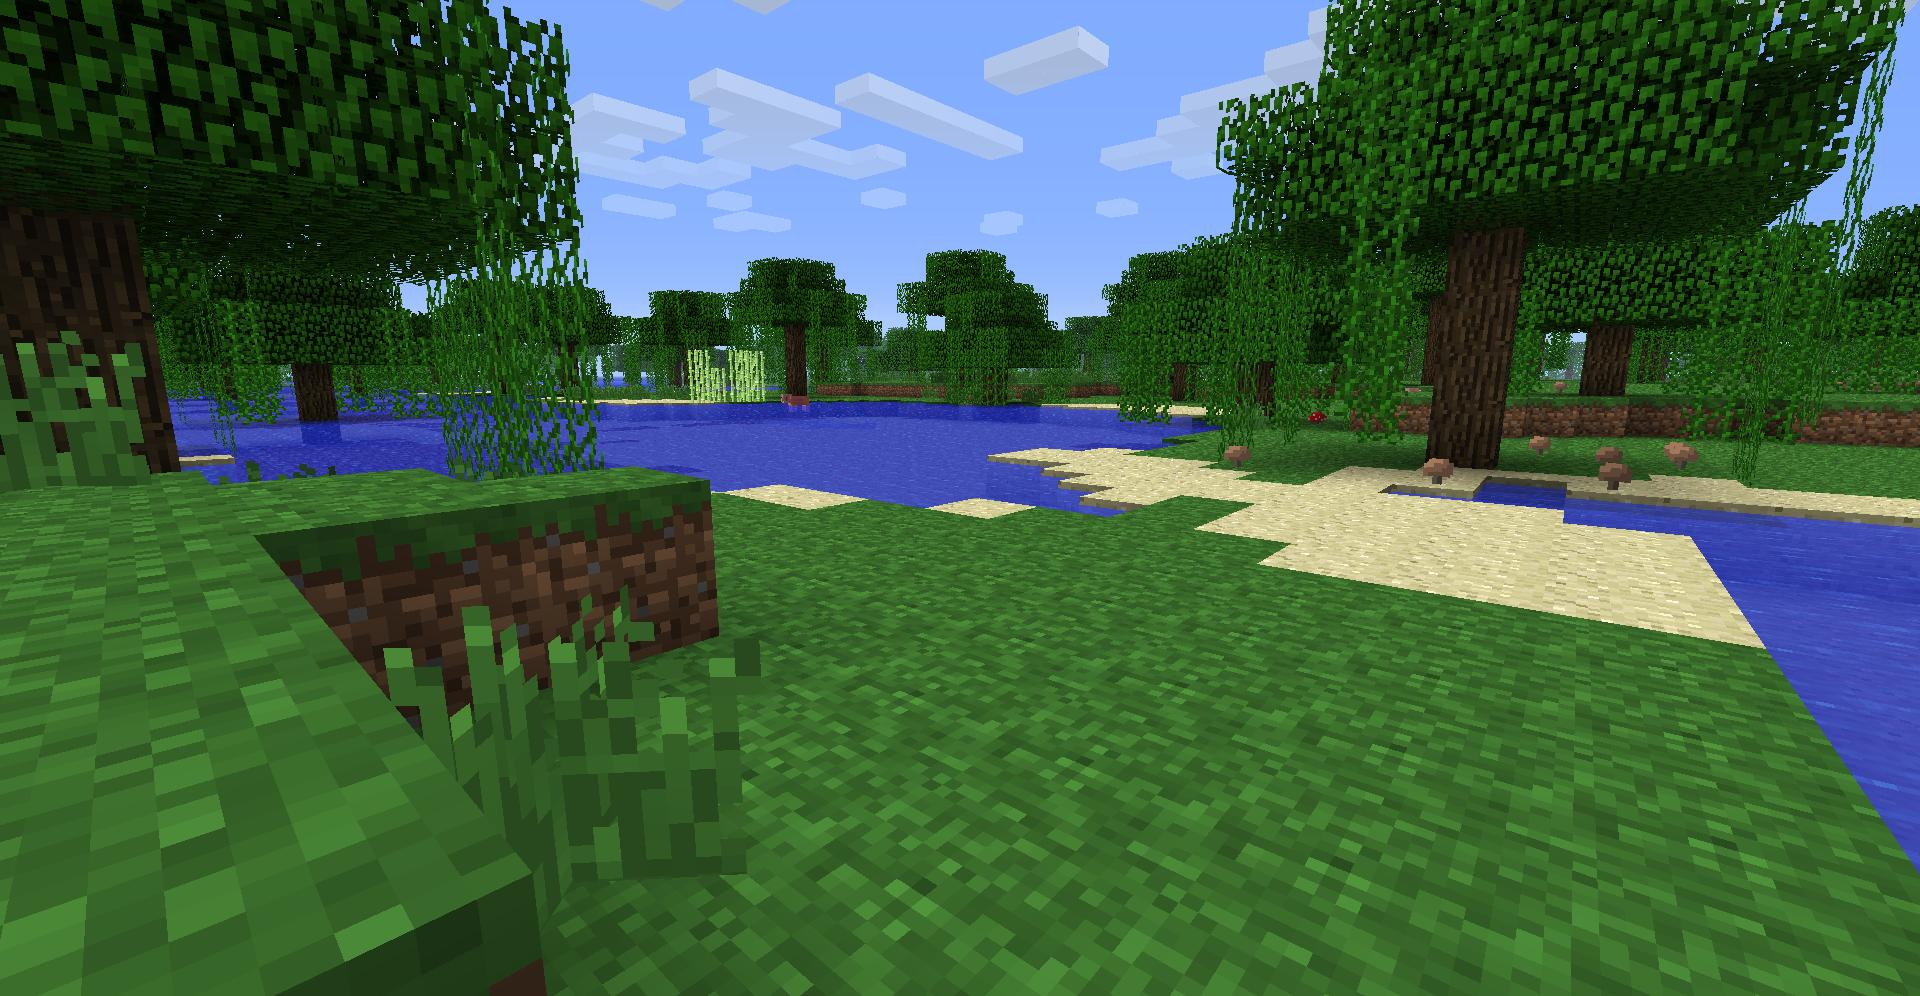
\includegraphics[width=8cm]{Images/InitialResearch/MCTerrainGeneration.jpg} \\
                        Example of Minecraft's terrain generation in a Swamp Biome \\ 
                        \vspace{0.2cm}

                        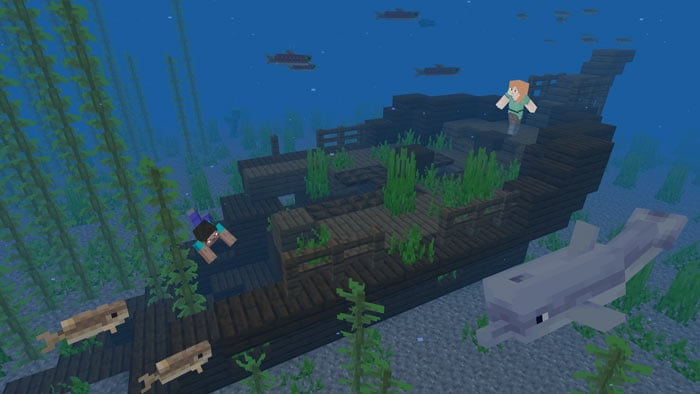
\includegraphics[width=8cm]{Images/InitialResearch/MCStructureGeneration.jpg} \\ 
                        Example of a Sunken Pirate Ship Structure \\
                        \vspace{0.2cm}
                        \end{center}
                        \vspace{0.2cm}

                        Minecraft itself is too complex and dynamic to be solved by current Machine Learning algorithms, along with there is no quantifiable 
                        metric for performance due to it's sandbox nature. There exist data sets for Minecraft, in the form of captured gameplay footage, but
                        there has been little to no success of quantifiably good solutions to solving Machine Learning problems within Minecraft. \\

                        \vspace{0.2cm}

                        Overall I feel like it would be good to borrow elements from Minecraft's terrain generation, such as its utilisation of Perlin Noise.
                        But the majority of the games systems are way too complex for a Machine Learning algorithm to solve. \\

                        \vspace{1cm}
                    \paragraph{Conway's Game of Life} \mbox{} \\
                        \vspace{0.2cm}
                        Conway's Game of Life is whats called a Cellular Automaton, which is a discrete computation model formed from a grid of cells along with 
                        a ruleset. Conway's is commonly referred to a Zero Player Game, where the input for the Automaton is defined at the start, with no
                        further adjustment needed for it to run. The game is fully Turing complete and can simulate a Universal Constructor. \\
                        \vspace{0.2cm}
                        The rules of Conway's are such that: \\

                        
                        \begin{center}
                            \normalsize
                            1. Any live cell with fewer than two live neighbours dies, as if by underpopulation. \\
                            2. Any live cell with two or three live neighbours lives on to the next generation. \\
                            3. Any live cell with more than three live neighbours dies, as if by overpopulation. \\
                            4. Any dead cell with exactly three live neighbours becomes a live cell. \\
                        \end{center}

                        \vspace{0.2cm}
                        It is rather interesting that such complicated Machines can be formed from such a simple ruleset, as an example 
                        here is a Turing Machine formed from 34 Thousand Cells: \\

                        \vspace{0.5cm}
                        \centerline{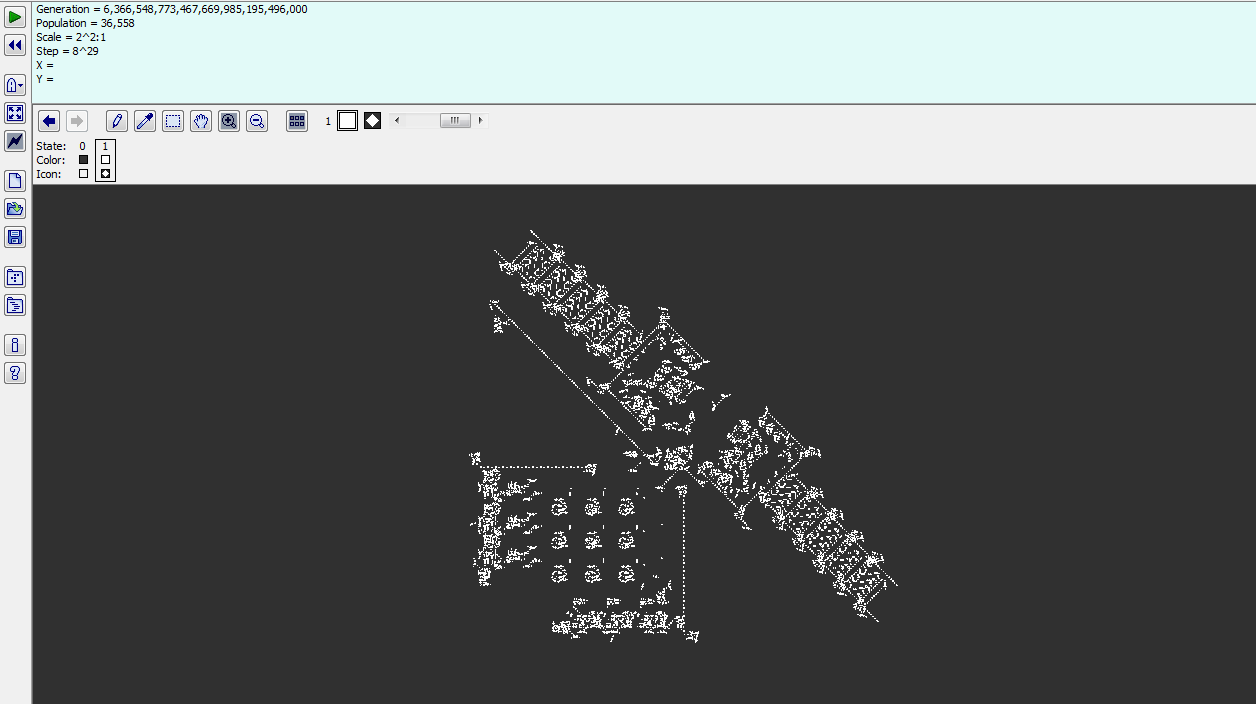
\includegraphics[width=14cm]{Images/InitialResearch/ConwaysTuringMachine.png}}
                        \vspace{0.2cm}

                        Overall, I think this shows that my simulation doesnt need to have complex rules in order to achieve 
                        interesting results. Conway's is formed from 4 simple rules, and yet is Turing complete.

                    \vspace{1cm}
                \subsubsection{Algorithms and Potential Data Types}
                    \large
                    \vspace{0.2cm}
                    \paragraph{Neural Network and Matrices} \mbox{} \\
                        As part of developing a Machine Learning Algorithm, I will need to implement a Matrix class in order to
                        implement a Neural Network. Matrices are commonly used to represent individual layers of a network. Along
                        with making calculations much easier, condensing them into performing operations on matrices, rather than
                        nested using nested for loops and lists. As part of my Initial Research I have taken the time to understand
                        how a Neural Network functions, it turns out I have already learned most of the Maths needed to understand
                        how it works in my A Level Maths and Further Maths courses. \\
                        \vspace{0.2cm}
                        A Neural Network functions as a series mathematical equations used to recognise relationships between inputs
                        and desired outputs. They take in a Vector of Input Data, and output a Vector of Output Data. They can be
                        in simple terms as a function: $N(x)$ where: $\{x \in V, N(x) \in V\}$. The functions name in this case is
                        Forward Propagation. \\
                        \vspace{0.2cm}
                        We form a Neural Network with multiple layers of Nodes, the layers being referred to as the Input Layer, 
                        Hidden Layer/s and Output Layer. In this case each Node is connected to every Node in the previous layer and
                        the following layer. In the below image is represented a Neural Network with a layer structure of $[3, 5, 2]$.

                        \vspace{0.1cm}
                        \centerline{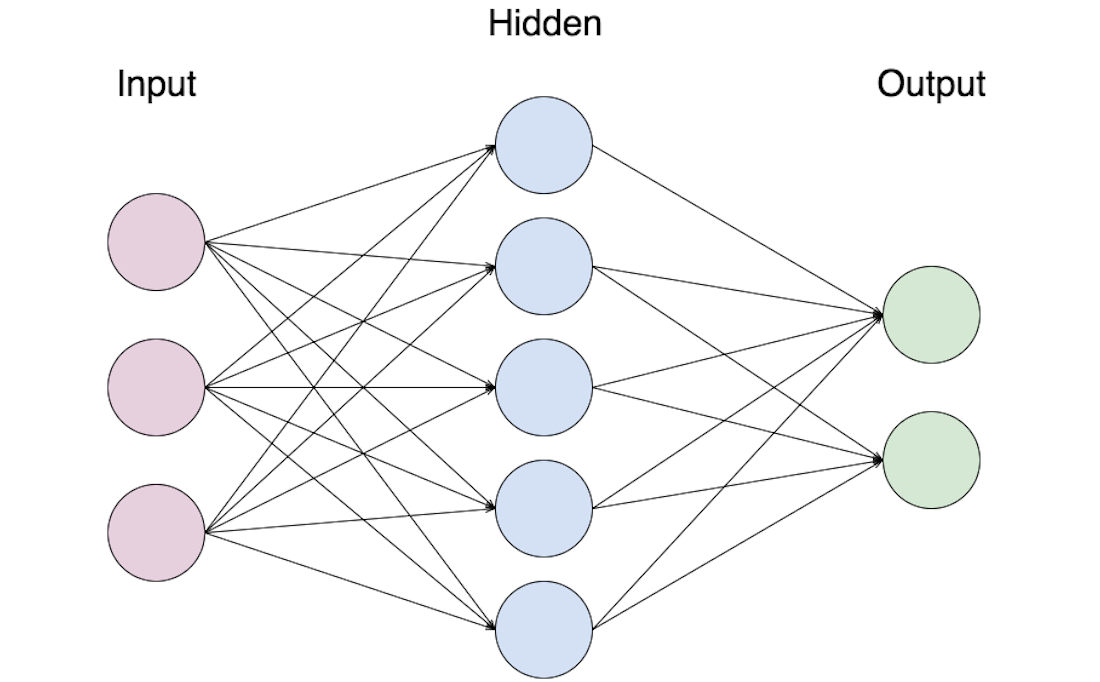
\includegraphics[width=10cm]{Images/InitialResearch/NeuralNetworkExample.png}}

                        Each connection, otherwise known as an Arc or Edge, has an associated weight. Along with every output of a
                        layer having an associated Bias. These are used to compute the outcome of a network. \\
                        \vspace{0.2cm}
                        Forward Propagation is used to compute the outcome of a network, it has a general form and uses 
                        Matrix Multiplication and Addition to achieve this.
                        \vspace{0.2cm}
                        
                        \begin{center}
                            $
                            S^{(L)} = 
                            \begin{bmatrix}
                            s^{(L)}_{0} \\
                            s^{(L)}_{1} \\
                            \vdots      \\
                            s^{(L)}_{n} 
                            \end{bmatrix}
                            = 
                            \begin{bmatrix}
                            w^{(L-1)}_{0,0} & w^{(L-1)}_{0,1} & \hdots  & w^{(L-1)}_{0,m} \\
                            w^{(L-1)}_{1,0} & w^{(L-1)}_{1,1} & \hdots  & w^{(L-1)}_{1,m} \\
                            \vdots          & \vdots          & \ddots  & \vdots          \\
                            w^{(L-1)}_{n,0} & w^{(L-1)}_{n,1} & \hdots  & w^{(L-1)}_{n,m} \\
                            \end{bmatrix}
                            \begin{bmatrix}
                            a^{(L-1)}_{0} \\
                            a^{(L-1)}_{1} \\
                            \vdots      \\
                            a^{(L-1)}_{n} 
                            \end{bmatrix}
                            +
                            \begin{bmatrix}
                            b^{(L)}_{0} \\
                            b^{(L)}_{1} \\
                            \vdots      \\
                            b^{(L)}_{n} 
                            \end{bmatrix}
                            $ 
                        \end{center}
                        
                        \begin{center}
                            $
                            \sigma(S^{(L)})
                            =
                            \sigma\left(
                            \begin{bmatrix}
                            s^{(L)}_{0} \\
                            s^{(L)}_{1} \\
                            \vdots      \\
                            s^{(L)}_{n} 
                            \end{bmatrix}
                            \right)
                            =
                            \begin{bmatrix}
                            \sigma(s^{(L)}_{0}) \\
                            \sigma(s^{(L)}_{1}) \\
                            \vdots              \\
                            \sigma(s^{(L)}_{n}) 
                            \end{bmatrix}
                            $ 
                        \end{center}
                        
                        \vspace{0.2cm}
                        We then apply an activation function as shown above, in this case we will apply the Sigmoid function: $\sigma(x)$ to $S^{(L)}$. 
                        The Sigmoid function is a Mathematical Function which \textit{squishes} values between 0 and 1. Shown Below:
                        
                        \begin{center}
                            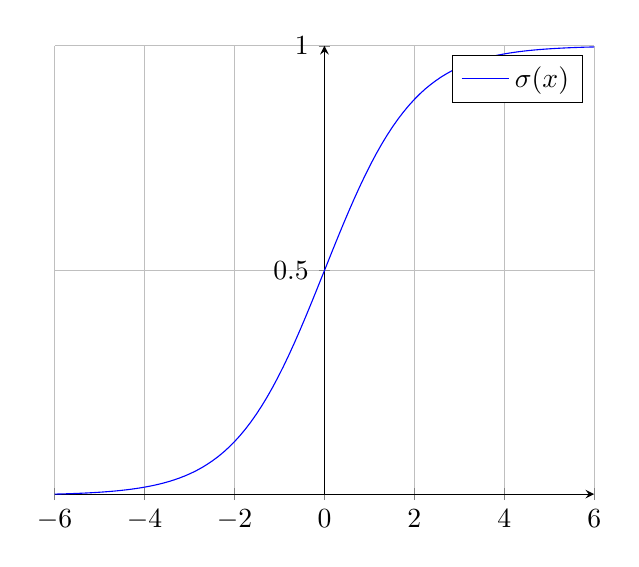
\begin{tikzpicture}[declare function={sigma(\x)=1/(1+exp(-\x));}]
                            \begin{axis}%
                            [
                                grid=major,     
                                axis x line=bottom,
                                ytick={0,.5,1},
                                ymax=1,
                                axis y line=middle,
                                samples=100,
                                domain=-6:6,
                                range=0:1
                                legend style={at={(1,0.9)}}     
                            ]
                                \addplot[blue,mark=none]   (x,{sigma(x)});
                                \legend{$\sigma(x)$}
                            \end{axis}
                            \end{tikzpicture}
                        \end{center}

                        Matrices can be used for all parts of a Neural Network implementation, and will prove very useful in my Technical
                        Solution. \\
                        \vspace{0.5cm}
                        
                        \pagebreak
                    \paragraph{Procedural Generation} \mbox{} \\
                        \vspace{0.2cm}
                        For my project I am going to have to procedurally generate 2d terrain, while researching this I came across a few algorithms
                        which seemed to be able to do this pretty well. I will compare two algorithms I discovered below.
                        
                        \begin{center}
                            \begin{tabular}{| C{6cm} | C{6cm} |}
                                \hline
                                {\Large Post-Processing Algorithms} & {\Large Perlin Noise} \\
                                \hline
                                I discovered two post processing algorithms often used for simple 2d terrain generation. 1 Averages squares 
                                around the selected square, and the other pulls it up or down the gradient its currently on.
                                I find these interesting because they're relatively simple, and I'm not quite sure whether they will produce good results or not. 
                                \vspace{0.2cm}\linebreak
                                So it would be interesting to test out implementing these in my prototype.
                                &
                                Perlin Noise is an algorithm developed by Ken Perlin for use in the digital generation of noise.
                                This noise can be combined to create \textit{realistic} looking height maps for world generation.
                                Perlin Noise retains continuity and is seeded so the generation can be entirely controlled.
                                By "retains continuity" I mean that you can sample the same point and retrieve the same value. 
                                \vspace{0.2cm}\linebreak
                                
                                If I was to implement Perlin noise it would take longer, but also might end up with a better result
                                due to it being more widely used. It's a trade-off between time to implement and desired result. \\
                                \hline
                            \end{tabular}
                        \end{center}
                        
                        I also discovered an algorithm called Poisson Disc Sampling, this can be used to sample random points 
                        in N dimensional space. It takes in 2 values, the R and K value, these values determine the output of
                        the function. The R values is the minimum distance a point has to be from another, randomly placed point
                        which hasn't been selected yet. If the distance between any existing points is less than R, the point
                        will be rejected and another will be selected. The K value determines how many rejected are needed before 
                        the algorithm will stop attempting to choose a new point.
                        
                        \vspace{0.5cm}
                    \paragraph{Proposed Programming Language and Associated Libraries} \mbox{} \\
                        \vspace{0.2cm}
                        When selecting a Programming Language and associated Graphical Libraries I took into consideration a few options.
                        Below I have weighed up 3 options for Programming Language, along with 2 graphical libraries per language
                        
                        \begin{flushleft}
                            \begin{longtable}{|M{2cm}|M{2cm}|M{8cm}|}
                            \hline
                            Proposed Solution & \multicolumn{2}{M{10cm}|}{Benefits and Downsides of Proposed Solution} \\
                            \hline
                                Python & \multicolumn{2}{M{10cm}|}{Python is the first thought which comes to mind when I think about programming, 
                                it is my favourite language and I'm yet to find anything which I prefer. Its very versatile and great
                                for rapid prototyping, the dynamic typing makes It great for coding quickly without worrying too
                                much about whether you're using a \textit{float32 or float64}. It also has hundreds of libraries
                                and is very well supported by its developers and the community.}\\
                            \hline
                                \multirow{2}*{\minitab[c]{Python \\ Graphical \\ Libraries}} & Pygame & Pygame is a highly customizable and well developed binding of
                                \textit{Simple DirectMedia Layer} (SDL) Library. It has a full set of 2d drawing tools, along with keyboard and audio
                                capabilities. I have lots of experience with Pygame so I already have code which I can take from, which will speed up
                                development when dealing with the Pygame library.\\
                            \cline{3-3}
                                &Tkinter & Tkinter provides an interface to the standard \textit{Tcl/Tk GUI Toolkit}, which is available
                                for most platforms, this makes it highly versatile. Though as my project is not intended as a software
                                package I dont see this as being an incredibly big selling point. Tkinter will serve mostly the same
                                purpose as Pygame but give me easier options for Graphical Input, I dont currently plan to add GUI so 
                                this feature isnt neccesary.\\
                            \hline
                                C\# & \multicolumn{2}{M{10cm}|}{C\# is my second favourite language, I have plenty of experience with it from developing games
                                with Unity. It's faster than Python and is less abstracted, but this speed isn't necessarily required
                                for my project. With C\# I could utilise the \textit{Unity Game Engine} for my project, but then
                                I might end-up relying on builtin types and functions rather than developing my own.}\\
                            \hline
                        \end{longtable}

                        \pagebreak
                        \begin{longtable}{|M{2cm}|M{2cm}|M{8cm}|}
                            \hline
                            Proposed Solution & \multicolumn{2}{M{10cm}|}{Benefits and Downsides of Proposed Solution} \\
                            \hline
                                \multirow{2}*{\minitab[c]{C\# \\ Graphical \\ Libraries}} & Windows Forms & Windows Forms is a relatively simple drag drop
                                interface for designing your own applications. I've never used it before but I could utilise it with C\# to create my project.
                                I belive it might be a bit overkill for my needs though, as it includes many, many UI features which I will have no use for.\\
                            \cline{3-3}
                                & WPF & WPF or \textit{Windows Presentation Foundation} is a versatile development platform for desktop applications.
                                It is relatively versatile in its uses and utilises XAML and is the UI Language of Windows Platforms. XAML would be a
                                new language for me to learn but I have experience with HTML so I dont believe it would be too difficult.
                                The platform would provide a stable base to my project.\\
                            \hline
                                Rust & \multicolumn{2}{M{10cm}|}{Rust is low level language designed for speed and efficiency, I started using it recently
                                as a side hobby and would like to use it more in future projects of mine. Though I feel like it may be a bit overkill for a Computer 
                                Science NEA, with it often being used for server side applications rather than general purpose applications.}\\
                            \hline
                                \multirow{2}*{\minitab[c]{Rust \\ Graphical \\ Libraries}} & Piston2d & Piston2d is a feature complete 2d graphics library which utilises OpenGl,
                                I've worked with it briefly before and I believe it would be a good option over Pixels if I needed more complex drawing
                                methods.\\
                            \cline{3-3}
                                & Pixels & Pixels is a lightweight 2d graphics library designed to simply push pixels to the screen, Its relatively simple
                                and i've used it for making a simple \textit{Falling Sand Game} before, could be a good little option if I wanted to develop
                                a lightweight solution.\\
                            \hline
                            \end{longtable}
                        \end{flushleft}
            \pagebreak
        \subsection{Prototype}
            \subsubsection{Prototype Objectives}
            \large
            \vspace{0.2cm}
            Before starting my Prototype I had to decide upon a short list of objectives I wanted to 
            complete/investigate as part of it. These boiled down to a few things:

            \vspace{0.2cm}
            \begin{enumerate}
                \item Terrain Generation
                \item Displaying the Generated Terrain using a Graphics Library
                \item Matrix and Vector implementation
            \end{enumerate}
            \vspace{0.2cm}

            For my Prototype, I first created a GitHub Repository, available here: 
            
            \vspace{0.1cm}
            \centerline{\textit{https://github.com/TheTacBanana/CompSciNEAPrototype}}
            \vspace{0.1cm}

            I had created a hierarchy of importance for development in my head, visualized using this flow diagram:

            \begin{center}
                \begin{tikzpicture}
                    \matrix (m)[matrix of nodes, column  sep=0.5cm,row  sep=0.5cm, align=center, nodes={rectangle,draw, anchor=center} ]{
                        |[block]| Creating a window with Graphics Library &  |[block]| Display Generated Terrain \\   
                        |[block]| Generate Terrain using a pseudorandom algorithm &  |[block]| Store Terrain to 2d List \\
                        |[block]| Create a Matrix Data Structure & |[block]| Create a Vector Data Structure which inherits from Matrix \\
                        |[block]| Create Operation Methods for the Data Structure & \\
                    };
                    \path [>=latex,->] (m-1-1) edge (m-1-2);
                    \path [>=latex,<-] (m-1-2) edge (m-2-2);
                    \path [>=latex,->] (m-2-1) edge (m-2-2);
                    \path [>=latex,->] (m-3-1) edge (m-3-2);
                    \path [>=latex,->] (m-3-1) edge (m-4-1);
                \end{tikzpicture}
            \end{center}

            I decided to use Python for developing my Prototype, this seemed like a good fit due to me 
            having lots of experience with the language. Python is a Dynamically Typed and Interpretted 
            language which makes it versatile for protyping and fast, iterative development.
            
            \vspace{0.5cm}
            \subsubsection{Terrain Generation and Displaying to Window}
            \vspace{0.25cm}

            Starting from the begining of my hierarchy I installed Pygame using \textit{pip} and started creating a window.
            This was a relatively simple task only taking a few lines:
            \vspace{0.5cm}

            \normalsize
            \begin{minted}[frame=leftline,framesep=2mm,baselinestretch=1.2,fontsize=\footnotesize,linenos]{python}
import pygame

simSize = 128
gridSize = 2

window = pygame.display.set_mode((simSize*gridSize, simSize*gridSize))
pygame.display.set_caption("Procedural Generation")

running = True
while running == True:
  for event in pygame.event.get():
    if event.type == pygame.QUIT:
      running = False
            \end{minted}

            \vspace{0.5cm}

            \large
            This creates a window like this: \\ 
            \vspace{0.5cm}
            \centerline{
\includegraphics{Images/Prototype/CreateWindowExample.PNG}}

            \vspace{0.5cm}

            Following the hierarchy I then added noise generation by generating random numbers and 
            assigning them to a 2d List. Shown here: 
            
            \begin{minted}[frame=leftline,framesep=2mm,baselinestretch=1.2,fontsize=\footnotesize,linenos]{python}
def GenerateMap(self, seed):
    random.seed(seed)
    for y in range(0, self.arraySize):
        for x in range(0, self.arraySize):
            self.heightArray[x][y] = round(random.random(),2)
            \end{minted}

            \vspace{0.5cm}

            \large
            After creating some code to draw squares based upon the random value, I ended up with this 
            random array of Black-White squares:\\
            \vspace{0.5cm}
            \centerline{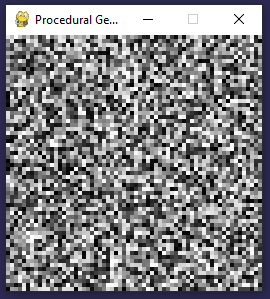
\includegraphics{Images/Prototype/RandomNoiseExample.PNG}}

            \vspace{0.5cm}

            This was a good start, but didnt really look like terrain yet. As part of my research I came 
            across simple algorithms to turn random noise into usable 2d terrain. I decided to implement
            these algorithms. They are relatively short and didnt take too much time to implement. I've
            named the two algorithms UpDownNeutralGen and Average.

            \vspace{1cm}

            \paragraph{UpDownNeutralGen Method} \mbox{} \\
            \vspace{0.25cm}

            The UpDownNeutralGen method takes a tile, and considers every tile around it. It sums the tile 
            which are greater than, less than, or within a certain range of the tile height. And then pulls
            the selected tile in the direction which has the highest precedence. As an example, here are some
            randomly generated values:

            \begin{center}
                \begin{tabular}{| C{0.75cm} | C{0.75cm} | C{0.75cm} |}
                    \hline
                    0.71 & 0.19 & 0.3 \\ [0.75cm]
                    \hline
                    0.46 & 0.26 & 0.82 \\ [0.75cm]
                    \hline
                    0.63 & 0.35 & 0.05 \\ [0.75cm]
                    \hline
                \end{tabular}
            \end{center}

            If we count the surrounding values into corresponding Higher, Lower and Neutral we get: \\

            \begin{center}
                \begin{tabular}{| M{2cm} | M{2cm} | M{2cm} |}
                    \hline
                    Higher & Lower & Neutral \\ [0.25cm]
                    \hline
                    4 & 1 & 3 \\ [0.25cm]
                    \hline
                \end{tabular}
            \end{center}

            \vspace{0.5cm}

            This leads us to calculating the \textit{pullValue}, respectively for each case:
            \begin{center}
                $Up -> pullValue = upTiles * 0.09$ \\
                $Down -> pullValue = upTiles * -0.08$ \\
                $Neutral -> pullValue = 0$ \\
                \vspace{0.5cm}
                $Value[x][y] \pluseq pullValue$\\
            \end{center}
            
            \vspace{0.5cm}

            We then add the pullValue to the original square value, leaving us with the updated value. The code for 
            this shown under the Prototype Code Header.
            \vspace{0.5cm}

            \paragraph{Average Method} \mbox{} \\
            \vspace{0.25cm}

            The Average method takes a tile and considers every tile around it, this time instead of looking at the
            differences, it creates an average from the 8 surrounding tiles. It then sets the selected tile to this
            average value. As an example, here are some randomly generated values:

            \begin{center}
                \begin{tabular}{| C{0.75cm} | C{0.75cm} | C{0.75cm} |}
                    \hline
                    0.83 & 0.93 & 0.64 \\ [0.75cm]
                    \hline
                    0.07 & 0.38 & 0.21 \\ [0.75cm]
                    \hline
                    0.33 & 0.94 & 0.95 \\ [0.75cm]
                    \hline
                \end{tabular}
                \vspace{0.25cm}

                Summing these and dividing by the total grants us the average:

                \[
                \frac{0.83 + 0.93 + 0.64 + 0.07 + 0.38 + 0.21 + 0.95 + 0.33 + 0.94}{9} = 0.586
                \]
                $Value[x][y] = 0.586$
            \end{center}
            \vspace{0.25cm}

            The code for this shown under the Prototype Code Header.

            \vspace{1cm}
            \subsubsection{Finished Terrain Generation}
            \vspace{0.25cm}

            Overall I am happy with the Terrain generation, though I feel as if it could be improved to look more realistic.
            The difference between the original random noise and the Colour Mapped Terrain looks so much better.

            \begin{center}
                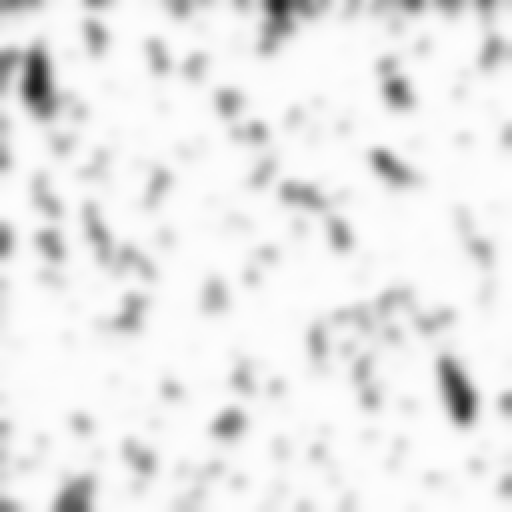
\includegraphics[width=6cm]{Images/Prototype/Seed420 Grayscale.png}
                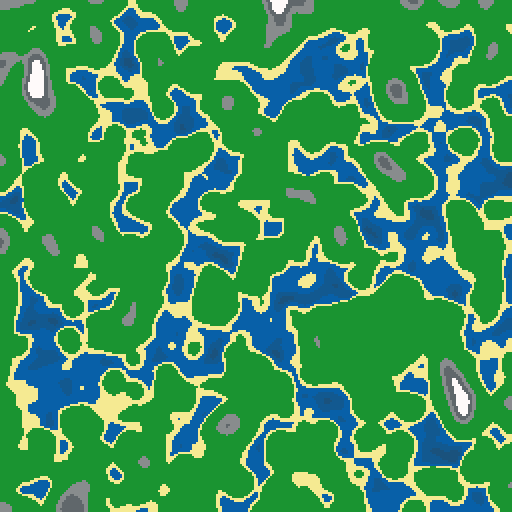
\includegraphics[width=6cm]{Images/Prototype/Seed420 Colour.png} 
            \end{center}
            
            \vspace{1cm}
            \subsubsection{Matrix Data Structure}
                \vspace{0.25cm}

                As part of my Matrix Class I made a list of operations which would be key to a Matrix Class, along with being useful
                for Machine Learning. A Matrix is an abstract data type, commonly used in Maths, but has practical uses in the world
                of Computer Science. It holds a 2d array of values such as: \\ 
                \begin{center}
                $\begin{pmatrix}
                    a & b\\
                    c & d
                \end{pmatrix}$ 
                $\begin{pmatrix}
                    a & b & c \\
                    d & e & f \\
                    g & h & i 
                \end{pmatrix}$ 
                $\begin{pmatrix}
                    a \\
                    b \\
                    c  
                \end{pmatrix}$ 
                $\begin{pmatrix}
                    a & b & c & d\\
                    e & f & g & h
                \end{pmatrix}$ 
                \end{center}
                The values in a Matrix can be manipulated using common operations such as $+ - *$ as long as the orders of the 2 Matrices
                match up. Along with other, non-standard operations which have other purposes.

                \vspace{0.25cm}
                As part of my Matrix Class, I implemented the following operators:
                \begin{enumerate}
                    \item Addition/Subtraction \\
                        Implementing Addition didnt take too long, I utilised a nested for loop to iterate over every value in both Matrices.
                        Adding the two values together into a temporary Matrix which the method then returned. 
                        \vspace{0.25cm}
                        \begin{center}
                            $\begin{pmatrix}
                                a & b\\
                                c & d
                            \end{pmatrix} +
                            \begin{pmatrix}
                                e & f\\
                                g & h
                            \end{pmatrix} =
                            \begin{pmatrix}
                                a+e & b+f\\
                                c+g & d+h
                            \end{pmatrix}$
                        \end{center}
                        \vspace{0.25cm}

                    \item Multiplication \\
                        Multiplication of Matrices is slightly more complicated, it is of $O(n^3)$ complexity, utilising a triple nested for loop.
                        It multiplies the row of a $M1$, by the column in $M2$. Summing the calculation into the element in the new Matrix $M3$. \\
                        
                        \vspace{0.25cm}
                        \begin{center}
                            $\begin{pmatrix}
                                a & b\\
                                c & d
                            \end{pmatrix} *
                            \begin{pmatrix}
                                e & f\\
                                g & h
                            \end{pmatrix} =
                            \begin{pmatrix}
                                a*e + b*g & a*f + b*h\\
                                c*e + d*g & c*f + d*h
                            \end{pmatrix}$
                        \end{center}
                        There is also Scalar Multiplication which multiples each value of a Matrix by the Scalar.
                        \begin{center}
                            $k *
                            \begin{pmatrix}
                                a & b\\
                                c & d
                            \end{pmatrix} =
                            \begin{pmatrix}
                                ka & kb\\
                                kc & kd
                            \end{pmatrix}$
                        \end{center}
                        \vspace{0.25cm}

                    \item Determinant \\
                        Calculating the Determinant of an NxN Matrix is a recursive algorithm. With the base case being the Determinant of a 2x2
                        Matrix. When calculating the Determinant of a 3x3 Matrix you create a Matrix of Cofactors, and multiply each 
                        value by the corresponding value in the Sin Matrix (\textit{Formed from repeating 1's and -1's}). Summing the values from
                        a singular Row or Column will then give you the Determinant. For a 4x4 you simply calculate the Determinant of the corresponding
                        3x3's to get the Cofactors.
                        
                        \begin{center}
                            $
                            \begin{vmatrix}
                                a & b\\
                                c & d
                            \end{vmatrix} = 
                                a*d - b*c
                            $
                        \end{center}
                        \vspace{0.25cm}
                        \begin{center}
                            $\begin{vmatrix}
                                a & b & c \\
                                d & e & f \\
                                g & h & i 
                            \end{vmatrix}  = a*
                            \begin{vmatrix}
                                e & f\\
                                h & i
                            \end{vmatrix}
                            -b*
                            \begin{vmatrix}
                                d & f\\
                                g & i
                            \end{vmatrix}
                            +c*
                            \begin{vmatrix}
                                d & e\\
                                g & h
                            \end{vmatrix}$
                        \end{center}
                        \vspace{0.25cm}

                    \item Dot Product \\
                        The Dot Product occurs between two vectors, and can be used to calculate the angle between them. 
                        Its a relatively simple operation only taking a few lines of code.
                        \begin{center}
                            $
                            \begin{pmatrix}
                                a \\
                                b \\
                                c
                            \end{pmatrix} .
                            \begin{pmatrix}
                                d \\
                                e \\
                                f
                            \end{pmatrix} = 
                            a*d + b*e + c*f$
                        \end{center}
                \end{enumerate}
                \vspace{1cm}
            \subsubsection{Prototype Evaluation}
                \vspace{0.2cm}
                Overall I am happy with my prototype, though I feel like some parts need to be improved. I did meet my 
                objectives for my prototype but there were improvements which can me made when I create my Technical Solution. 
                Namely the Terrain Generation along with the Matrix class. I feel that Perlin noise would be a better alternative
                to the two algorithms I used. In theory it should produce better results, and also provide more marks for 
                complexity. My Matrix class could be rewritten to be more efficient, along with using operator overloading, which
                I didnt know Python could do at the time. I also feel like having Vector inherit from Matrix is relatively pointless,
                there is no need for it when I could just use 1 wide Matrices instead.
        \subsection{Second Interview}
            \vspace{0.2cm}
            I asked a few more questions to my Expert regarding my project at this point. Receiving feedback on my Prototype and gaining a
            greater understanding of the Machine Learning Model I'm intending to use. \\
            \vspace{0.2cm}

            \begin{enumerate}
                \item What are your thoughts on my prototype? \\ 
                    \vspace{0.2cm}
                    "I think your prototype is good, but could be improved. The use of Operator Overloading would improve your Matrix Class,
                    and optimising some of your algorithms would be useful. The Terrain generation looks good, but I think its a bit
                    water heavy, this is where Perlin Noise might help you to achieve better results. Would also be more fine tunable to
                    your liking."

                \item Is a Dual Neural Network a good model to choose? \\
                    \vspace{0.2cm}
                    "A Dual Neural Network should in theory be a complex enough Model for your project. The concern I have is whether your
                    Network will be able to generalise enough in order to sufficiently 'solve' the simulation you design. There are some
                    algorithms you could implement in order to tackle this though. You could do some research into these before finalising 
                    your design."

                \item Which Activation Functions should I implement? \\
                    \vspace{0.2cm}
                    "The most commonly used are Sigmoid, TanH, ReLu and SoftMax. They are relatively simple so wont take long to implement.
                    Those would be a good starting point for testing your Neural Network."
                
                \item What type of Reward system should I use? \\
                    \vspace{0.2cm}
                    "As far as I'm aware there are two types of reward systems, Sparse and Dense. I think that Sparse would be better suited
                    to your project. Sparse is where the reward given to the Agent is 0 for most actions. Compared to dense where reward
                    is given for most most actions."
            \end{enumerate}

            \pagebreak
        \subsection{Objectives}
            \large
            Taking into account my Prototype and Interview, I have formed a list of objectives I feel to be most 
            appropriate for my Investigation.\\
            \vspace{0.2cm}
            If all completed they will form a complete solution which will answer my Investigations question.
            Below is the list of objectives split into 6 key sections:

            \subsubsection*{User Input}
                \begin{enumerate}
                    \item Read Parameters from a Json formatted file
                    \item Check Parameters fall within a certain range to prevent errors
                    \item Give user option to load Neural Network Training progress
                \end{enumerate}
            \subsubsection*{Simulation}
                \begin{enumerate}
                    \item Utilise Perlin Noise to generate a 2d List of terrain heights
                    \item Store Terrain Heights in a Tile Data Type
                    \item Utilise Threading to generate Terrain Faster
                    \item Display terrain to a window
                    \item Map ranges of terrain heights to specific colour bands
                    \item Utilise Poisson Disc Sampling to generate objects for the Agent to interact with
                    \item Implement enemies which use basic pathfinding to traverse towards the player
                    \item Generate multiple enemies upon starting the simulation
                    \item Allow the enemies to attack the Agent
                \end{enumerate}   
            \subsubsection*{Agent}
                \begin{enumerate}
                    \item Implement Movement options for the Agent
                    \item Implement the ability to pick up the generated Objects
                    \item Implement the ability to attack the generated enemies
                    \item Create methods to sample the terrain around the Agent
                    \item Create methods to convert the sampled Tiles into a grayscale input vector for a neural network
                    \item Create reward methods to reward the agent given the terrain samples and action
                \end{enumerate}   
            \subsubsection*{Matrix Class}
                \begin{enumerate}
                    \item Implement a Dynamic Matrix Class with appropriate Operations such as:
                        \begin{enumerate}
                            \item Multiplication
                            \item Addition
                            \item Subtraction
                            \item Transpose
                            \item Sum
                            \item Select Row/Column
                        \end{enumerate}
                    \item Create appropriate errors to throw when utilising methods the incorrect way
                \end{enumerate}   
            \subsubsection*{Deep Reinforcement Learning}
                \begin{enumerate}
                    \item Dynamically create a Dual Neural Network model based upon loaded parameters
                    \item Implement an Abstract Class for Activation Functions
                    \item Implement Activation Functions inheriting from the Abstract Class such as:
                    \begin{enumerate}
                        \item Sigmoid
                        \item TanH
                        \item ReLu
                        \item SoftMax
                    \end{enumerate}
                    \item Create methods to Forward Propagate the neural network
                    \item Create methods to calculate the loss of the network using the Bellman Equation
                    \item Create methods to Back Propagate calculated error through the neural network
                    \item Create methods to update weights and biases within the network to converge on a well trained network
                    \item Utilise the outlined Matrix class to perform the mathematical operations in the specified methods
                    \item Implement Load and Save Methods to save progress in training
                    \item Implement a Double Ended Queue/Deque Data Type
                    \item Implement Experience Replay utilising the Deque Data Type to increase training accuracy
                \end{enumerate}   
            \subsubsection*{Data Logger}
                \begin{enumerate}
                    \item Be able to create a Data Logger class to log data points across training
                    \item Be able to create a Data Structure for the Data Logger
                    \item Allow multiple types specified types for a single parameter
                    \item When adding a new Data Point the Logger will check it to make sure it matches the given Data Structure
                    \item Implement a Heap Data Type
                    \item Implement a Heap sort using the Heap Data Type
                    \item Be able to sort by a parameter in the Data Structure
                    \item Be able to select a single parameter from the data points
                    \item Implement Load and Save Functions to save progress during training
                \end{enumerate}   
        \subsection{Modelling of the Problem}
            \large
            \vspace{0.2cm}
            In this section I will define and derive all the Mathematical Formulae relating to my Project. This includes all the Matrix Operations 
            I plan to use and the General Forms of Forward Propagation and Back Propagation. \\
            \vspace{0.2cm}

            \subsubsection{Matrices}
                \paragraph{Overview} \mbox{} \\
                Matrices are a Mathematical Data Structure, storing elements in the shape of a Rectangle. They are arranged Rows and Columns.
                An $m$ x $n$ Matrix will have $m$ Rows and $n$ Columns. \\
                \vspace{0.2cm}
                As part of defining the Matrix Operations, below is defined Matrix $A$ and Matrix $B$ and can be of any size. \\
                \vspace{0.5cm}

                \begin{center}
                    $
                    A = 
                    \begin{bmatrix}
                        a_{1,1} & a_{1,2} & \hdots  & a_{1,m} \\
                        a_{2,1} & a_{2,2} & \hdots  & a_{2,m} \\
                        \vdots  & \vdots  & \ddots  & \vdots  \\
                        a_{n,1} & a_{n,2} & \hdots  & a_{n,m} \\
                    \end{bmatrix}
                    $
                \end{center}
                \vspace{0.2cm}
                \begin{center}
                    $
                    B = 
                    \begin{bmatrix}
                        b_{1,1} & b_{1,2} & \hdots  & b_{1,m} \\
                        b_{2,1} & b_{2,2} & \hdots  & b_{2,m} \\
                        \vdots  & \vdots  & \ddots  & \vdots  \\
                        b_{n,1} & b_{n,2} & \hdots  & b_{n,m} \\
                    \end{bmatrix}
                    $
                \end{center}

                \paragraph{Matrix Addition} \mbox{} \\
                    \vspace{0.2cm}
                    Matrix Addition is the Operation of adding two Matrices by adding the Corresponding Elements together. Matrix Addition is Commutative. 
                    Below is A added to B. \\

                    \begin{center}
                        $
                        A + B =
                        \begin{bmatrix}
                            a_{1,1} + b_{1,1} & a_{1,2} + b_{1,2} & \hdots  & a_{1,m} + b_{1,m} \\
                            a_{2,1} + b_{2,1} & a_{2,2} + b_{2,2} & \hdots  & a_{2,m} + b_{2,m} \\
                            \vdots            & \vdots            & \ddots  & \vdots            \\
                            a_{n,1} + b_{n,1} & a_{n,2} + b_{n,2} & \hdots  & a_{n,m} + b_{n,m} \\
                        \end{bmatrix}
                        $
                    \end{center}

                \paragraph{Matrix Subtraction} \mbox{} \\
                    \vspace{0.2cm}
                    Matrix Subtraction is the Operation of subtracting two Matrices by adding the Corresponding Elements together, with the 2nd Matrix's element 
                    being Negated. Below is B Subtracted from A. \\

                    \begin{center}
                        $
                        A - B =
                        \begin{bmatrix}
                            a_{1,1} - b_{1,1} & a_{1,2} - b_{1,2} & \hdots  & a_{1,m} - b_{1,m} \\
                            a_{2,1} - b_{2,1} & a_{2,2} - b_{2,2} & \hdots  & a_{2,m} - b_{2,m} \\
                            \vdots            & \vdots            & \ddots  & \vdots            \\
                            a_{n,1} - b_{n,1} & a_{n,2} - b_{n,2} & \hdots  & a_{n,m} - b_{n,m} \\
                        \end{bmatrix}
                        $
                    \end{center}

                \paragraph{Matrix Multiplication} \mbox{} \\
                    \vspace{0.2cm}
                    Matrix Multiplication calculates the Dot Product between the Rows in Matrix $A$ and Columns in Matrix $B$. The Dot Product is a Vector Operation
                    which takes two equal-length series of Numbers and returns a single Number. Each element in the 1st series of Numbers is Multiplied with the opposing element
                    in the 2nd series, these are then summed to find the Dot Product. \\

                    \begin{center}
                        $
                        AB = 
                        \begin{bmatrix}
                            c_{1,1} & c_{1,2} & \hdots  & c_{1,m} \\
                            c_{2,1} & c_{2,2} & \hdots  & c_{2,m} \\
                            \vdots  & \vdots  & \ddots  & \vdots  \\
                            c_{n,1} & c_{n,2} & \hdots  & c_{n,m} \\
                        \end{bmatrix}
                        $
                    \end{center}
                    \vspace{0.2cm}
                    \begin{center}
                        Such that \[ c_{i,j} = a_{i,1}b_{1,j} + a_{i,2}b_{2,j} + \hdots + a_{i,n}b_{n,j} = \sum^{n}_{k=1}a_{i,k}b_{k,j} \]
                    \end{center}

                \paragraph{Matrix Scalar Multiplication} \mbox{} \\
                    \vspace{0.2cm}
                    Scalar Multiplication Multiplies each element by a single Scalar, in this case $k$. \\

                    \begin{center}
                        $
                        k * A = 
                        \begin{bmatrix}
                            ka_{1,1} & ka_{1,2} & \hdots  & ka_{1,m} \\
                            ka_{2,1} & ka_{2,2} & \hdots  & ka_{2,m} \\
                            \vdots  & \vdots  & \ddots  & \vdots  \\
                            ka_{n,1} & ka_{n,2} & \hdots  & ka_{n,m} \\
                        \end{bmatrix}
                        $
                    \end{center}

                \paragraph{Matrix Hadamard Product} \mbox{} \\
                    \vspace{0.2cm}
                    The Hadamard Product calculates the element-wise product between two equally sized Matrices. \\

                    \begin{center}
                        $
                        A \odot B =
                        \begin{bmatrix}
                            a_{1,1}b_{1,1} & a_{1,2}b_{1,2} & \hdots  & a_{1,m}b_{1,m} \\
                            a_{2,1}b_{2,1} & a_{2,2}b_{2,2} & \hdots  & a_{2,m}b_{2,m} \\
                            \vdots         & \vdots         & \ddots  & \vdots         \\
                            a_{n,1}b_{n,1} & a_{n,2}b_{n,2} & \hdots  & a_{n,m}b_{n,m} \\
                        \end{bmatrix}
                        $
                    \end{center}

                \paragraph{Matrix Transpose} \mbox{} \\
                    \vspace{0.2cm}
                    The Transpose of a Matrix flips the given Matrix over the Diagonal, effectively Rows become Columns. \\

                    \begin{center}
                        $
                        B^{T} = 
                        \begin{bmatrix}
                            b_{1,1} & b_{2,1} & \hdots  & b_{n,1} \\
                            b_{1,2} & b_{2,2} & \hdots  & b_{n,2} \\
                            \vdots  & \vdots  & \ddots  & \vdots  \\
                            b_{1,m} & b_{2,m} & \hdots  & b_{n,m} \\
                        \end{bmatrix}
                        $
                    \end{center}
                    
            \subsubsection{Forward Propagation}
                \paragraph{Overview} \mbox{} \\
                    \vspace{0.2cm}
                    Forward Propgation is used in a Neural Network to calculate the output of the Network. It feeds Input Data through each
                    Layer, leaving each Node with its resultant Activation Value. This is completed in two processes: Pre-Activation and Activation. \\
                    \vspace{0.4cm}
                    \centerline{The Standard Notation I will be using to describe the Calculations:}

                    \vspace{0.2cm}
                    \begin{addmargin}[2em]{0em}                     
                        $a^{(L)}_{i} = $ The Activation Value for the $i^{th}$ Node in the $L^{th}$ Layer \\
                        $z^{(L)}_{i} = $ The Pre-Activation Value for the $i^{th}$ Node in the $L^{th}$ Layer \\
                        $w^{(L)}_{m,n} = $ The Weight between node $n \rightarrow m$ from the $L^{th}$ to the $(L + 1)^{th}$ \\
                        $b^{(L)}_{i} = $ The Bias Value for the $i^{th}$ Node in the $L^{th}$ Layer \\
                    \end{addmargin}
                    \vspace{0.4cm}

                \paragraph{Pre-Activation} \mbox{} \\
                    \vspace{0.2cm}
                    The Pre-Activation Value for the $i^{th}$ Node is the Sum of the Preceding Layers Activation Values, Multiplied by the Weight value
                    between them. This then has the Bias Value added. $M$ is the size the Layer $(L - 1)$.

                    \vspace{0.2cm}
                    \begin{center}
                        \[ z^{(L)}_{i} = \sum_{k=1}^{M}(a^{(L-1)}_{i} \times w^{(L-1)}_{k,i}) + b^{(L)}_{i} \]
                    \end{center}
                    \vspace{0.4cm}

                    This can also be represented in its Matrix Form rather easily. You take the Vector of Activation Values from $(L - 1)$ and multiply
                    it by the Weight Matrix from $(L - 1)$. You then add the Vector of Bias Values and that leaves you with the Pre-Activation for Layer
                    $L$.

                    \begin{center}
                        \[ Z^{(L)} = W^{(L-1)} \times A^{(L-1)} + B^{(L)}\]
                    \end{center}
                    \vspace{0.2cm}
                    \begin{center}
                        \[
                        Z^{(L)} = 
                        \begin{bmatrix}
                        z^{(L)}_{0} \\
                        z^{(L)}_{1} \\
                        \vdots      \\
                        z^{(L)}_{n} 
                        \end{bmatrix}
                        = 
                        \begin{bmatrix}
                        w^{(L-1)}_{0,0} & w^{(L-1)}_{0,1} & \hdots  & w^{(L-1)}_{0,m} \\
                        w^{(L-1)}_{1,0} & w^{(L-1)}_{1,1} & \hdots  & w^{(L-1)}_{1,m} \\
                        \vdots          & \vdots          & \ddots  & \vdots          \\
                        w^{(L-1)}_{n,0} & w^{(L-1)}_{n,1} & \hdots  & w^{(L-1)}_{n,m} \\
                        \end{bmatrix}
                        \begin{bmatrix}
                        a^{(L-1)}_{0} \\
                        a^{(L-1)}_{1} \\
                        \vdots      \\
                        a^{(L-1)}_{n} 
                        \end{bmatrix}
                        +
                        \begin{bmatrix}
                        b^{(L)}_{0} \\
                        b^{(L)}_{1} \\
                        \vdots      \\
                        b^{(L)}_{n} 
                        \end{bmatrix}
                        \]
                    \end{center}
                    \vspace{0.2cm}

                \paragraph{Activation} \mbox{} \\
                    \vspace{0.2cm}
                    Activation Functions are usually an abstraction representing the rate of "Action Potential" firing in the Node.
                    The most Common Activations for Neural Networks are the following 3 Activations: \\
                \paragraph{ReLu} \mbox{} \\
                    \begin{center}
                        \[
                            \text{ReLu}(x) =  \begin{cases}
                                                x < 0 & 0 \\
                                                x > 0 & x
                                                \end{cases}
                        \]
                        
                        \vspace{0.2cm}
                        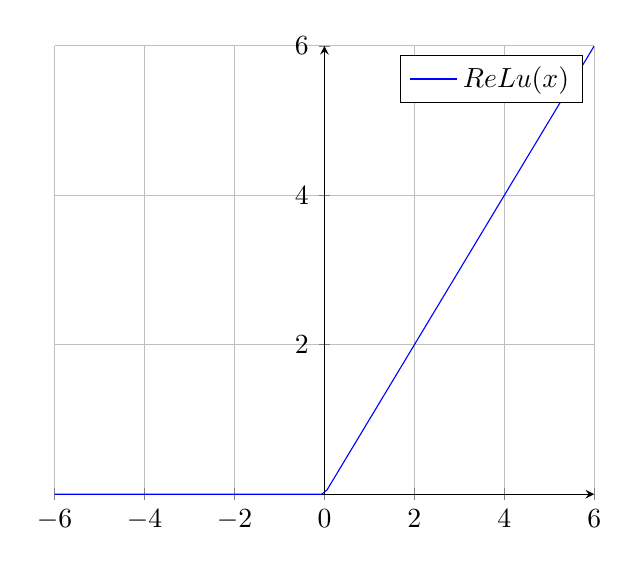
\begin{tikzpicture}[declare function={ReLu(\x)=max(0, x);}]
                        \begin{axis}
                            [
                                grid=major,     
                                axis x line=bottom,
                                ytick={0,2,4,6},
                                axis y line=middle,
                                samples=100,
                                domain=-6:6,
                            ]
                            \addplot[blue,mark=none]   (x,{ReLu(x)});
                            \legend{$ReLu(x)$}
                        \end{axis}
                        \end{tikzpicture}
                    \end{center}

                \paragraph{Sigmoid} \mbox{} \\
                    \begin{center}
                        Sigmoid$(x) = $ \mathLarge{\frac{1}{1 + e^{-x}}} \\
                        \vspace{0.2cm}
                        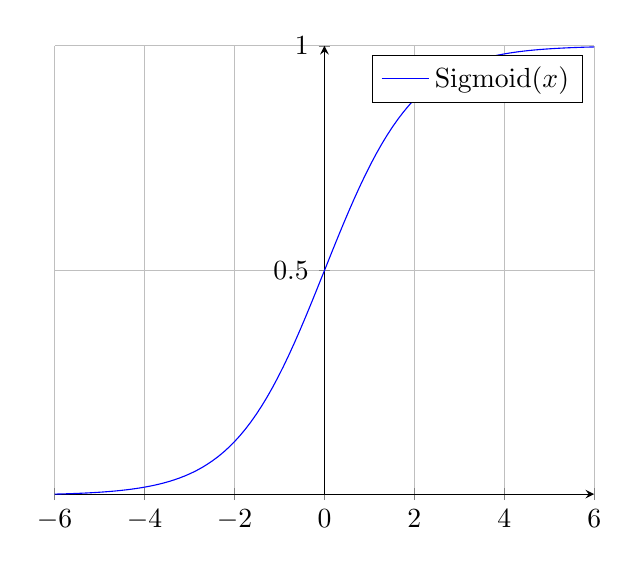
\begin{tikzpicture}[declare function={sigma(\x)=1/(1+exp(-\x));}]
                        \begin{axis}
                            [
                                grid=major,     
                                axis x line=bottom,
                                ytick={-1,-.5,0,.5,1},
                                ymax=1,
                                axis y line=middle,
                                samples=100,
                                domain=-6:6,
                                range=-1:1
                                legend style={at={(1,0.9)}}     
                            ]
                                \addplot[blue,mark=none]   (x,{sigma(x)});
                                \legend{Sigmoid$(x)$}
                        \end{axis}
                        \end{tikzpicture}
                    \end{center}

                \paragraph{TanH} \mbox{} \\
                    \begin{center}
                        TanH$(x) = $ \mathLarge{\frac{\sinh(x)}{\cosh(x)}} $ = $ \mathLarge{\frac{e^{x} - e^{-x}}{e^{x} + e^{-x}}} \\
                        \vspace{0.4cm}
                        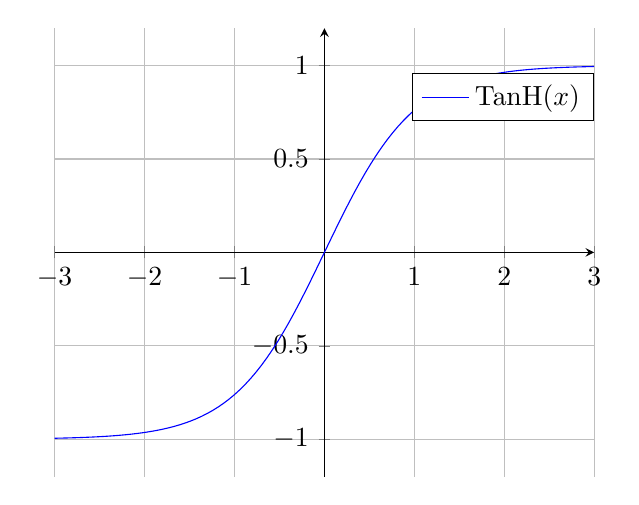
\begin{tikzpicture}[declare function={TanH(\x)=(exp(\x) - exp(-\x))/(exp(\x) + exp(-\x));}]
                        \begin{axis}
                            [
                                grid=major,     
                                axis x line=middle,
                                ytick={-1,-.5,0,.5,1},
                                axis y line=middle,
                                samples=100,
                                domain=-3:3,
                                ymax=1.2,
                                ymin=-1.2,
                                legend style={at={(1,0.9)}}     
                            ]
                                \addplot[blue,mark=none] (x,{TanH(x)});
                                \legend{TanH$(x)$}
                        \end{axis}
                        \end{tikzpicture}
                    \end{center}

                \paragraph{SoftMax} \mbox{} \\
                    SoftMax is an exception to the Activation Functions and is a Generalisation of Sigmoid to Multiple Dimensions. It
                    takes in a Vector \textbf{z} of $K$ Real Numbers, and normalises it into a probability distribution which Sums to 1. \\ 

                    \begin{center}
                        \begin{math}
                            \text{SoftMax}(\textbf{z})_{i} = \mathLarge{\frac{e^{z_{i}}}{\sum_{j=1}^{K} e^{z_{j}}}}
                        \end{math} \\
                        \vspace{0.2cm}
                        For $i = 1, \hdots,K$ And \textbf{z} $ = (z_{1},\hdots,z_{K})$ \\
                    \end{center}
                    
            \subsubsection{Differentiation}
                \paragraph{Differentiation from First Principles}  \mbox{} \\
                    \vspace{0.2cm}
                    Differentiation is the process of finding the Gradient of a Function at a specific point. In the case of a Neural Network,
                    this can be used to measure the sensitivity of the Function Output, in respect to the Input. This derivative is known as said 
                    Functions' Gradient Function. \\
                    \vspace{0.2cm}
                    
                    With a simple straight line graph we can find the gradient as {\Large$\frac{\Delta y}{\Delta x}$, $\Delta$} (Delta) is used to 
                    represent a fininite increment. \\
                    \vspace{0.2cm}

                    When find the Derivative of a more Complex Function we can use Two Points. Point $P : (x, f(x))$ and Point $Q : (x + h, f(x + h))$.
                    The variable $h$ tends towards 0, so Points $Q$ will eventually be ontop of point $P$. This is called Differentiation from First
                    Principles.
                    \vspace{0.4cm}

                    \begin{eqnarray*}
                        \frac{\Delta y}{\Delta x} &=& \lim_{h\to0} \left(\frac{f(x + h) - f(x)}{(x + h) - x}\right) \\
                        &=& \lim_{h\to0} \left(\frac{f(x + h) - f(x)}{h}\right)
                    \end{eqnarray*}
                    \vspace{0.6cm}

                    Derivatives are more commonly represented as $f'(x)$ or $\frac{dy}{dx}$

                    \vspace{0.4cm}
                \paragraph{Standard Differentiation Rules}  \mbox{} \\
                    \vspace{0.2cm}
                    Instead of manually using Smaller and Smaller Values of $h$ manually, there are standard Differentiation Rules. These are as follows: \\
                    \vspace{0.4cm}

                    \begin{eqnarray*}
                        y = x^{k} &\rightarrow& \frac{dy}{dx} = kx^{k-1} \\
                        y = k &\rightarrow& \frac{dy}{dx} = 0 \\
                        y = e^{kx} &\rightarrow& \frac{dy}{dx} = ke^{kx} \\
                        y = f(x)g(x) &\rightarrow& f(x)g'(x) + f'(x)g(x) \\
                        f(x) = \frac{g(x)}{h(x)} &\rightarrow& f'(x) = \frac{g'(x)h(x) - g(x)h'(x)}{h(x)^{2}} \\
                    \end{eqnarray*}
                    \vspace{0.4cm}

                    These rules are applied to each component of the Function to find the Derivative. 

                \paragraph{Chain Rule}  \mbox{} \\
                    \vspace{0.2cm}
                    The Chain Rule is used to compute the derivative of Nested Functions such as $f(x) = g(h(x))$. The derivative of this Function can be expressed as: \\
                    \vspace{0.4cm}

                    \[f'(x) =  g'(h(x))h'(x)\]

                    \vspace{0.4cm}

                    This can be applied to an infinite number of Functions, where $f(x) = g_{1}(g_{2}(\hdots(g_{n}(x))))$. By this rule we can represent the derivative as
                    a Series of Derivatives Multiplied together:

                    \[
                        \frac{df}{dx} = \frac{df}{df_{1}} \frac{df_{1}}{df_{2}} \frac{df_{2}}{df_{3}} \hdots \frac{df_{n}}{df_{x}}
                    \]

                \paragraph{Partial Derivatives}  \mbox{} \\
                    \vspace{0.2cm}
                    Partial Derivatives are used when the Function in question contains Multiple Variables. They utilise the same rules, except the Variables
                    which aren't being derived get treated as constants. The Derivative of $f(x, y)$ with respect to $x$ is expressed as $f_{x}'(x,y)$ or 
                    {\Large $\frac{\partial f}{\partial x}$}. 

            \subsubsection{Back Propagation}
                \paragraph{Overview} \mbox{} \\
                    \vspace{0.2cm}
                    Back Propagation is the algorithm used to adjust Weights and Bias' in a Neural Network. Through using this algorithm you can successfully "train"
                    the Network to recognise certain patterns in data. The Input Data gets propagated through the Network using Forward Propagation, and then the output
                    is passed into the Loss Function.

                \paragraph{The Bellman Equation} \mbox{} \\
                    \vspace{0.2cm}
                    The Bellman Equation is a method of optimisation, and is used for dynamic programming. In the context of Machine Learning we can utilise it
                    to reinforce good behaviour and negate bad behaviour. By writing the relationships between two states in the form of an action, we can optimise this
                    by choosing the best action when given a state. If we let $s_{t}$ be the current state, we can define all the possible actions from that state as
                    $a_{t} \in \Gamma(s_{t})$. Where $\Gamma(s_{t})$ represents all given actions from a state. We can also define the State Transition from $s_{t} \to s_{t+1}$ 
                    as $T(s_{t}, a)$ when action $a$ has been taken. The Reward from this is given as $R(s_{t}, a)$. A Discount Factor $0 < \gamma < 1$ is also defined to assume
                    impatience, compounding the effects of $\gamma$ the further in the future the Reward is. \\
                    \vspace{0.2cm}
                    With these definitions, an infinite-horizon problem is formed: \\

                    \[ V(s_{0}) = \max_{\{a_{t}\}_{t=0}^{\infty}} \sum_{t=0}^{\infty} \gamma^{t} \cdot R(s_{t},a_{t}) \]
                    \vspace{0.2cm}

                    We can form this into another Equation which uses the Principle of Optimality, such that: \\
                    \vspace{0.2cm}

                    \begin{center}
                        \textit{An optimal policy has the property that whatever the initial state and initial decision are, the remaining decisions must constitute an 
                        optimal policy with regard to the state resulting from the first decision.} - Richard E. Bellman
                    \end{center}
                    \vspace{0.2cm}

                    We will consider the first decision seperately to all future reward, and then collect the future decisions within the brackets, which the infinite-horizon problem
                    above is equivalent too.

                    \[ \max_{a_{0}} \left\{ R(s_0, a_0) + \gamma \cdot \left[ \max_{\{a_{t}\}_{t=1}^{\infty}} \sum_{t=1}^{\infty} \gamma^{t-1} \cdot R(s_{t},a_{t})\right] \right\} \]
                    \vspace{0.2cm}

                    This at first glance has only made the problem uglier but infact has made our lives easier. It can be condensed further into a Recursively Defined Function:
                    \vspace{0.2cm}

                    \[ V(s_{0}) = \max_{a_{0}} \{ R(s_{0}, a_{0}) + \gamma \cdot V(x_{1}) \} \] 
                    \centerline{When subjected to: $ x_{1} = T(s_{0}, a_{0})$}
                    \vspace{0.2cm}

                \paragraph{Loss Function} \mbox{} \\
                    \vspace{0.2cm}
                    The Loss Function of a Network represents how well a Neural Network is performing. The aim of the Back Propagation is to minimise this Functions output. When using
                    a standard Neural Network and you're training on a labelled data set, you can be certain about the Expected Output. The standard Loss Function is as follows: \\ 
                    \vspace{0.2cm}
                    
                    \begin{eqnarray*}
                        Loss_{i} &=& \frac{1}{2} \cdot (Expected Output_{i} - Actual Output_{i})^{2} \\
                        &=& \frac{1}{2} \cdot (y_{i} - \hat{y}_{i})^{2}
                    \end{eqnarray*}
                    \vspace{0.2cm}

                    This is whats called the Half Square Difference. This Differentiates nicely which is why it is commonly used. \\
                    \vspace{0.2cm}

                    To finally use Bellman Equation as a Loss Function we need to convert it into a Loss Function: \\
                    \vspace{0.2cm}

                    \[Q(s_t, a_t) = R(s_t, a_t) + \gamma \cdot \max_{a_{t+1}} Q(s_{t+1}, a_{t+1})\]
                    \[Loss = \left( R(s_t, a_t) + \gamma \cdot \max_{a_{t+1}} Q(s_{t+1}, a_{t+1}) - Q(s_t, a_t) \right)^2\]

                \paragraph{Gradient Descent} \mbox{} \\ 
                    \vspace{0.2cm}   
                    To minimise the Loss Function, the Weights and Bias' in the Network need to be algorithmically adjusted to converge towards the expected outputs. You can
                    calculate these adjustments by using Partial Derivatives. You can take the Derivative of every Weight and Bias with respect to the Loss Function. The Derivatives
                    of each weight can vary, such as one weight being 0.5 and the other being 3, the Second Weight affects the Loss Function 10$\times$ as much. This process is
                    known as Gradient Descent. \\

                \paragraph{Differentiating Activation Functions} \mbox{} \\ 
                    \vspace{0.2cm}
                    As part of Back Propgation we need to derive all the Activation Functions we use within our Layer structure. The Derivatives are shown below. \\
                    \vspace{0.2cm}
                    The ReLu Derivative:
                    \vspace{0.2cm}
                    \[
                        \text{ReLu}(x) =  \begin{cases}
                                            0 & x < 0 \\
                                            x & x > 0
                                            \end{cases} 
                    \]
                    \[
                        \text{Relu'}(x) = \begin{cases}
                                            0 & x < 0 \\
                                            1 & x > 0
                                            \end{cases}
                    \]
                    \vspace{0.2cm}
                    \begin{center}
                        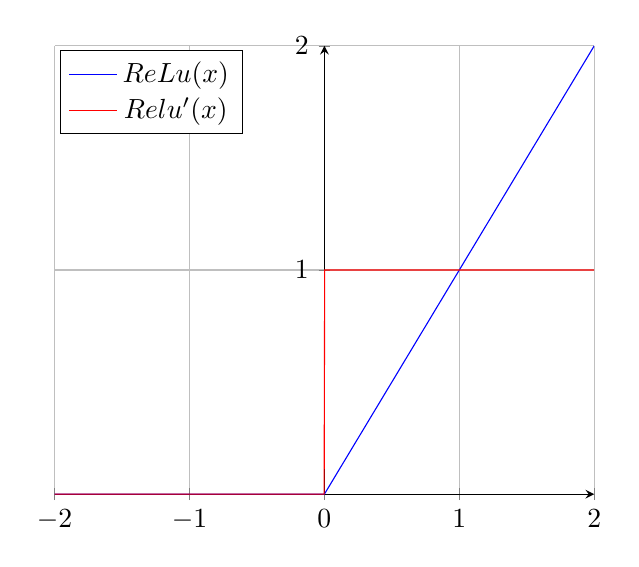
\begin{tikzpicture}[declare function={ReLu(\x)=max(0, x);}]
                        \begin{axis}
                            [
                                grid=major,     
                                axis x line=bottom,
                                ytick={0,1,2,3,4},
                                axis y line=middle,
                                samples=1000,
                                domain=-2:2,
                                legend style={at={(0.01,0.99)},anchor=north west},
                                ymax=2,
                                ymin=0,
                            ]
                            \addplot[blue,mark=none]   (x,{ReLu(x)});
                            \addplot [red,mark=none] {ifthenelse(x>0,1,0)};
                            \legend{$ReLu(x)$, $Relu'(x)$}
                        \end{axis}
                        \end{tikzpicture}
                    \end{center}

                    The Sigmoid Function Derivative:
                    \vspace{0.2cm}
                    \begin{eqnarray*}
                        \text{Sigmoid}(x) &=& \mathLarge{\frac{1}{1 + e^{-x}}} \\
                                            &=& (1 + e^{-x})^{-1} \\
                        \frac{d\sigma(x)}{dx}&=& -1 \cdot (1 + e^{-x})^{-2} \cdot -e^{-x} \\
                                            &=& \mathLarge{\frac{e^{-x}}{(1 + e^{-x})^{2}}} \\
                                            &=& \mathLarge{\frac{e^{-x}}{1 + e^{-x}} \cdot \frac{1}{1 + e^{-x}}} \\
                                            &=& \mathLarge{\frac{e^{-x} + 1 - 1}{1 + e^{-x}} \cdot \frac{1}{1 + e^{-x}}} \\
                                            &=& \left( \mathLarge{\frac{1 + e^{-x}}{1 + e^{-x}} - \frac{1}{1 + e^{-x}}} \right) \cdot \mathLarge{\frac{1}{1 + e^{-x}}} \\
                                            &=& \text{Sigmoid}(x) \cdot (1 - \text{Sigmoid}(x)) \\
                    \end{eqnarray*}
                    
                    \vspace{0.2cm}
                    \begin{center}
                        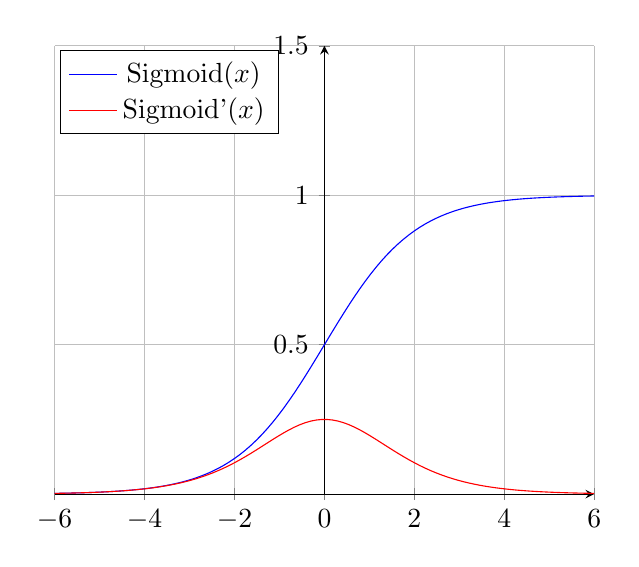
\begin{tikzpicture}[declare function={sigma(\x)=1/(1+exp(-\x));}, declare function={sigmaDer(\x)=sigma(\x)*(1 - sigma(\x));}]
                        \begin{axis}
                            [
                                grid=major,     
                                axis x line=bottom,
                                ytick={-1,-.5,0,.5,1, 1.5},
                                ymax=1.5,
                                ymin=0,
                                axis y line=middle,
                                samples=100,
                                domain=-6:6,
                                legend style={at={(0.01,0.99)},anchor=north west},
                            ]
                                \addplot[blue,mark=none]   (x,{sigma(x)});
                                \addplot[red,mark=none]   (x,{sigmaDer(x)});
                                \legend{Sigmoid$(x)$, Sigmoid'$(x)$}
                        \end{axis}
                        \end{tikzpicture}
                    \end{center}

                    The TanH Derivative:
                    \vspace{0.2cm}
                    \begin{eqnarray*}
                        \text{TanH}(x) &=& \mathLarge{\frac{\sinh(x)}{\cosh(x)}}  \\
                                        &=& \mathLarge{\frac{e^{x} - e^{-x}}{e^{x} + e^{-x}}} \\
                        \text{TanH'}(x)&=& \mathLarge{\frac{(e^{x} + e^{-x})(e^{x} + e^{-x}) - (e^{x} - e^{-x})(e^{x} - e^{-x})}{(e^{x} + e^{-x})^{2}}} \\
                                        &=& \mathLarge{\frac{(e^{x} + e^{-x})^{2}}{(e^{x} + e^{-x})^{2}} - \frac{(e^{x} - e^{-x})^{2}}{(e^{x} + e^{-x})^{2}}} \\
                                        &=& 1 - \text{TanH}^{2}(x) \\
                    \end{eqnarray*}
                    \vspace{0.2cm}

                    \begin{center}
                        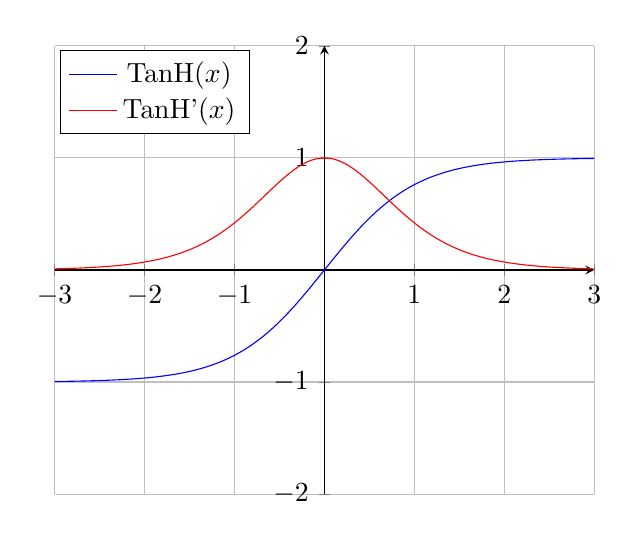
\begin{tikzpicture}[declare function={TanH(\x)=(exp(\x) - exp(-\x))/(exp(\x) + exp(-\x));}, declare function={TanHDer(\x)=1 - TanH(x)^2;}]
                        \begin{axis}
                            [
                                grid=major,     
                                axis x line=middle,
                                ytick={-2,-1,0,1,2},
                                axis y line=middle,
                                samples=100,
                                domain=-3:3,
                                ymax=2,
                                ymin=-2,
                                legend style={at={(0.01,0.99)},anchor=north west}    
                            ]
                                \addplot[blue,mark=none] (x,{TanH(x)});
                                \addplot[red,mark=none] (x,{TanHDer(x)});
                                \legend{TanH$(x)$, TanH'$(x)$}
                        \end{axis}
                        \end{tikzpicture}
                    \end{center}
\end{flushleft}